\subsection{The ecosystem: siblings are common, annotations are not enough}
Sibling operations are the norm in multi-tool servers: \PctServersGeTenEsc\,\% of the
\NumServersGeTen{} servers with at least ten tools contain an escalation-capable group, and
\NumReadDestructiveGroups{} groups put a read tool and a destructive tool on the same resource.
\PctReadOnlyHint\,\% of tools declare \texttt{readOnlyHint}, but \PctGroupsNoAnnotation\,\% of
sibling groups carry no annotation at all. Where annotations exist they agree with our
AI-assisted audit labels on read vs.\ write for \AnnRWAcc\,\% of tools, yet only \TrueDestructiveFlagged{} of the
\TrueDestructive{} audited tools those labels call destructive are flagged \texttt{destructiveHint}
and \TrueDestructiveNoAnn{} carry no annotation.
Table~\ref{tab:profiles} compares profilers: the zero-cost system profile (decisive annotations,
otherwise name rules) is as accurate as an LLM profiler and errs toward over- rather than
under-estimating severity, the safe direction for a guard.

\begin{table}[t]\centering\caption{Operation profilers against 300 tools labeled by an AI assistant, not human ground truth (\%). Under = severity underestimated, the unsafe direction.}\label{tab:profiles}
\footnotesize\setlength{\tabcolsep}{3pt}\begin{tabular}{lrrrr}\toprule
profiler & exact & $\kappa$ & read/write & under\\\midrule
name rules & 80.3 & 0.73 & 85.3 & 4.0\\
annot.\,+\,rules (system) & 83.7 & 0.77 & 92.0 & 3.3\\
Qwen3.5 LLM & 84.0 & 0.77 & 94.3 & 6.7\\
Gemma3\,+\,annot. (reference) & 82.3 & 0.75 & 93.0 & 3.0\\
\bottomrule\end{tabular}\end{table}


\subsection{RQ1: siblings are each other's nearest neighbours}
For the \NNTools{} grouped tools in the study pool, the most similar other tool on the same
server is one of its siblings \NNSibQwen\,\% of the time with Qwen3-Embedding
(\NNSibBge\,\% BGE, \NNSibMini\,\% MiniLM), against \NNChance\,\% expected by chance
(Fig.~\ref{fig:geometry}, left). Requests separate the target from its siblings by a thin
margin, and for \SibOutQwen\,\% of requests (\SibOutMini\,\% with MiniLM) a sibling
outscores the target outright (Fig.~\ref{fig:geometry}, right).

\begin{figure}[t]\centering
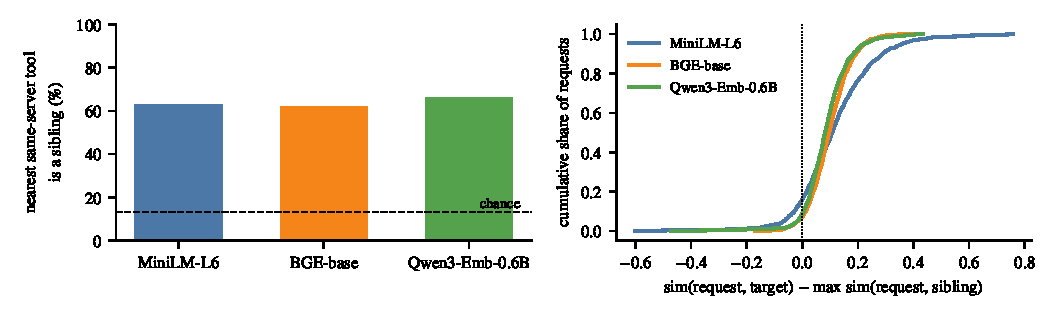
\includegraphics[width=\columnwidth]{../figs/geometry.pdf}
\caption{Left: share of grouped tools whose nearest same-server tool is a sibling.
Right: request-to-target minus request-to-best-sibling similarity; left of zero, a sibling wins.}
\label{fig:geometry}\end{figure}

\textbf{Answer to RQ1.} Siblings are far closer to each other than chance would place them, and a
sibling outscores the target for some requests outright, so a retriever alone cannot be relied on
to separate operations on the same resource.

\textbf{Approximate search is not the cause.} Exact search over \NumPoolTools{} tools takes
\FlatMs\,ms per request; HNSW at $ef{=}10$ loses \HnswTenDrop{} points of top-1 accuracy;
at $ef{=}100$ (\HnswMsHundred\,ms) it comes within 0.1 points, and it matches exact search only at
$ef{=}200$, where it is slower than exact search. Tool catalogs are too small
for ANN to matter.


\subsection{RQ2: how often selection escalates}
\textbf{Read requests routed to writes.} The primary safety outcome is a read request whose selected
tool would create, send, overwrite, start or delete something. Of the \ReadReqs{} requests whose target the reference classifies as read,
the retriever's top hit does this for \RWRet{} (\RWRetRate\,\%, 95\,\% CI \RWRetCI) at
\NumPoolTools{} tools, and Qwen3.5 selection over the top five for \RWQPlain{} (\RWQPlainRate\,\%,
\RWQPlainCI). Over all requests these are \RWRetAll\,\% and \RWQPlainAll\,\%. The read
denominator is robust: the name-rule profile used at generation calls 592 targets reads and
disagrees with the reference on 128, yet all \RWRet{} retriever and \RWQPlain{} Qwen3.5 violations
come from the 555 requests both call reads, so the rates move only between 2.17 and 2.52\,\%
and 0.31 and 0.36\,\%. Across the \EffPairs{} distinct
verified escalations at \NumPoolTools{} tools (retriever-only top-1 and all top-5 selection
runs), the first author tagged \EffTagged{} (the rest are classified by tool name) by what the picked tool would do
beyond the request: overwrite a value (\EffOverwrite), create a record (\EffCreate), start a
workflow, job or payment (\EffTrigger), delete or cancel (\EffDelete), send or submit (\EffSend),
other (\EffOther). Deletion accounts for \EffDelete{} of \EffPairs; most escalations change, add, start or send
something rather than remove it.

\textbf{Retriever-only routing.} The top-ranked tool is an escalation for
1.73\,\%, \GRNoneKConf\,\% and 1.59\,\% of requests at 200, 1,000 and 5,000 tools (verified; 95\,\% CI
\GRNoneKCI{} at 1,000) and \GRNonePoolConf\,\% at
\NumPoolTools{} (\GRNonePoolCI) with Qwen3-Embedding (Fig.~\ref{fig:retrieval}, middle). For the dense retrievers the automatic rate
rises with catalog size (Qwen3-Embedding 3.1 to 4.5\,\%, BGE 2.7 to 5.1\,\%), but the verified rate does not: the growth is
in false alarms. The shortlist itself is risky: \RetQwenKExpo\,\% of read requests at 1,000 tools
have an update or destructive tool in their top five. Table~\ref{tab:examples} shows typical
verified cases.

\begin{table}[t]\centering
\caption{Human-confirmed escalations (abridged requests; tool names as published).}\label{tab:examples}
\scriptsize\setlength{\tabcolsep}{2pt}
\begin{tabular}{p{0.42\columnwidth}p{0.23\columnwidth}p{0.29\columnwidth}}\toprule
request & target & selected instead\\\midrule
show all sites for my team, incl.\ deleted ones & \texttt{list\_sites} & \texttt{delete\_site}\\
show the stock symbols on my watchlist & \texttt{get\_watchlist} & \texttt{remove\_from\_\allowbreak watchlist}\\
list unpaid invoices, newest first & \texttt{getInvoices} & \texttt{deleteInvoice}\\
show my inbox webhook's status and URL & \texttt{get\_webhook} & \texttt{delete\_webhook}\\
preview the invoice filled with these values & \texttt{preview\_\allowbreak template} & \texttt{send\_invoice}\\
continue the price check: answer option c & \texttt{checker\_answer} & \texttt{submit\_enquiry}\\
\bottomrule\end{tabular}\end{table}


\begin{figure*}[t]\centering
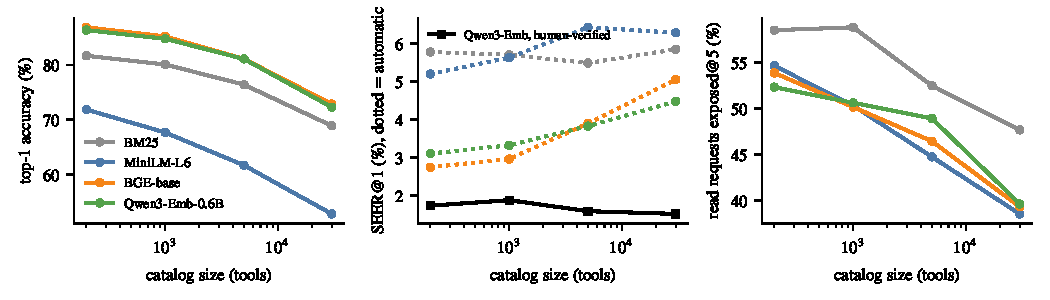
\includegraphics[width=0.85\textwidth]{../figs/retrieval.pdf}
\caption{Retriever-only routing versus catalog size: top-1 accuracy; side-effect escalation of
the top-1 tool, automatic (dotted, per retriever) and human-verified (black, Qwen3-Emb); and read
requests whose top-5 contains an update or destructive tool.}
\label{fig:retrieval}\end{figure*}

\textbf{LLM selection.} An LLM choosing among the top five removes most escalation
(Table~\ref{tab:main}). At \NumPoolTools{} tools Qwen3.5-9B escalates on \SelQPlainPoolConf\,\%
of requests (\SelQPlainPoolConfN{} of \NumQueries, 95\,\% CI \SelQPlainPoolCI), Gemma3-12B on
\SelGPlainPoolConf\,\%, Phi-4-14B on \SelPPlainPoolConf\,\% and Qwen3-1.7B on
\SelSPlainPoolConf\,\%, against \GRNonePoolConf\,\% (\GRNonePoolCI) for the retriever alone, all
verified: a 3.5- to 5.2-fold reduction. Counts per selector are small (\ConfNMin--\ConfNMax),
so we do not rank selectors. At 1,000 tools Qwen3.5 escalates on \SelQPlainKConf\,\%. Most selection errors are not side-effect errors at all. Of Qwen3.5's errors at
\NumPoolTools{} tools, \ErrMiss\,\% are retrieval misses (target not shortlisted),
\ErrOther\,\% pick a tool with the same operation on another server, \ErrNone\,\% answer
\texttt{NONE}, only \ErrSib\,\% pick a sibling, and the remaining 12\,\% pick an unrelated tool. Some cross-server picks are equally good answers: counting a tool with the same operation,
resource and severity on another server as correct adds 4.0 to 4.8 points of accuracy for every
selector and variant (coarse operation-equivalence, column \emph{any}). In an audit of \EquivN{} such picks by the first author (single rater), \EquivYes{}
(\EquivRate\,\%, 95\,\% CI \EquivCI\,\%) would serve the request as well; the rest were judged not
equivalent. Coarse equivalence therefore overstates functional correctness, and we
keep exact accuracy as the primary measure. These picks never count as escalations, since their
severity matches the target's, but that does not make them safe.

\begin{table}[t]\centering\caption{End-to-end selection at \NumPoolTools{} tools over the Qwen3-Emb shortlist (top five unless stated; \NumQueries{} requests). Acc.\ any: correct, or an equivalent tool (same operation, resource and severity) on another server; diagnostic only. Esc.\ auto: escalation by the automatic reference; verified: human-confirmed escalations; guard: verified escalations the any-increase guard would let through (it holds the share in \emph{held}). Tok.: mean selector-prompt tokens (intent call excluded). exp.+tags: expand+tags; matched: count-matched plain shortlist.}\label{tab:main}
\setlength{\tabcolsep}{1.6pt}\footnotesize
\begin{tabular}{llrrrrrrr}\toprule
 & & \multicolumn{2}{c}{accuracy} & \multicolumn{3}{c}{escalation (\%)} & & \\
selector & variant & exact & any & auto & verified & guard & held & tok.\\\midrule
Qwen3.5-9B & plain & 77.8 & 82.0 & 1.88 & 0.29 & 0.07 & 16.8 & 309 \\
Qwen3.5-9B & matched & 79.7 & 83.9 & 1.59 & 0.29 & 0.07 & 17.0 & 583 \\
Qwen3.5-9B & native & 78.8 & 82.8 & 2.09 & 0.36 & 0.07 & 17.0 & 350 \\
Qwen3.5-9B & tags & 78.5 & 82.5 & 2.38 & 0.36 & 0.07 & 17.2 & 350 \\
Qwen3.5-9B & expand & 80.7 & 85.1 & 1.52 & 0.22 & 0.14 & 17.2 & 575 \\
Qwen3.5-9B & exp.+tags & 81.1 & 85.4 & 1.44 & 0.22 & 0.14 & 16.6 & 632 \\
Qwen3.5-9B & sibling & 81.0 & 85.6 & 1.73 & 0.29 & 0.14 & 16.7 & 632 \\
Qwen3.5-9B & top-10 & 78.7 & 82.8 & 1.88 & 0.29 & 0.00 & 17.3 & 517 \\
Qwen3.5-9B & top-15 & 79.4 & 83.7 & 1.73 & 0.29 & 0.07 & 17.2 & 727 \\
\midrule
Gemma3-12B & plain & 74.0 & 78.8 & 2.53 & 0.36 & 0.07 & 14.9 & 319 \\
Gemma3-12B & matched & 73.2 & 78.6 & 2.45 & 0.72 & 0.29 & 14.4 & 608 \\
Gemma3-12B & tags & 74.5 & 79.1 & 1.95 & 0.22 & 0.07 & 14.6 & 360 \\
Gemma3-12B & sibling & 78.5 & 83.0 & 1.95 & 0.22 & 0.07 & 15.2 & 658 \\
\midrule
Phi-4 & plain & 75.6 & 79.6 & 2.02 & 0.43 & 0.07 & 15.5 & 302 \\
Phi-4 & matched & 73.9 & 77.6 & 1.66 & 0.14 & 0.07 & 14.9 & 574 \\
Phi-4 & sibling & 78.2 & 83.0 & 1.59 & 0.29 & 0.00 & 15.0 & 623 \\
\midrule
Qwen3-1.7B & plain & 74.2 & 78.9 & 2.67 & 0.43 & 0.07 & 19.6 & 310 \\
Qwen3-1.7B & matched & 74.0 & 78.4 & 1.73 & 0.14 & 0.07 & 19.6 & 583 \\
Qwen3-1.7B & tags & 74.4 & 79.0 & 1.80 & 0.14 & 0.00 & 18.8 & 352 \\
Qwen3-1.7B & sibling & 73.4 & 78.2 & 2.89 & 0.36 & 0.14 & 19.1 & 631 \\
\bottomrule\end{tabular}\end{table}

\begin{table}[t]\centering\caption{End-to-end selection at 1,000 tools over the Qwen3-Emb shortlist (top five unless stated; \NumQueries{} requests). Esc.\ auto: escalation by the automatic reference; verified: human-confirmed escalations; guard: verified escalations the any-increase guard would let through (it holds the share in \emph{held}). Tok.: mean selector-prompt tokens (intent call excluded). exp.+tags: expand+tags; matched: count-matched plain shortlist.}\label{tab:main1k}
\setlength{\tabcolsep}{1.6pt}\footnotesize
\begin{tabular}{llrrrrrr}\toprule
 & & \multicolumn{1}{c}{accuracy} & \multicolumn{3}{c}{escalation (\%)} & & \\
selector & variant & exact & auto & verified & guard & held & tok.\\\midrule
Qwen3.5-9B & plain & 91.1 & 0.51 & 0.07 & 0.00 & 17.7 & 313 \\
Qwen3.5-9B & native & 91.6 & 0.43 & 0.14 & 0.00 & 17.7 & 354 \\
Qwen3.5-9B & tags & 92.2 & 0.43 & 0.07 & 0.00 & 17.7 & 354 \\
Qwen3.5-9B & sibling & 94.2 & 0.36 & 0.07 & 0.00 & 17.6 & 553 \\
\midrule
\midrule
\midrule
\bottomrule\end{tabular}\end{table}


\textbf{Automatic severity scoring overstates escalation.} The reference flags \EscFlagged{} unique
(request, tool) pairs as escalations in the runs we report. The first author labeled them; on
\ConsFlagN{} the second author also labeled blind and the two then reached a consensus, which replaces
the first author's label. Only \EscTrue{} of \EscLabeled{} decided pairs are real (\EscPrec\,\%;
\EscUndecided{} undecided), so automatic scoring overstates escalation \EscOverstate-fold. The largest
group of false alarms (\EscFalseUpdDest) is an update tool against a sibling marked destructive,
typically because the server set \texttt{destructiveHint} on an ordinary overwrite. Of the real
escalations, \EscTrueFromRead{} start from a read request and \EscTrueToDelete{} end in a tool the
reference calls destructive. An earlier AI-assisted pass had confirmed \EscAITrue{} of the 178 pairs from the main runs; we use it
for no reported rate.

\textbf{Do automatic labels miss escalations?} Of the 30 sampled wrong picks the reference
did not flag (half from LLM selection, half from retriever-only routing), both raters answered
\IndUnN; the first author marked \IndUnAuthorYes{} of them as escalations and the second author none; after discussion the consensus
was none (0 of 15 per stratum; 95\,\% CI \MissSelCI\,\% each). Our main results are therefore \emph{verified} rates. As a sensitivity analysis we add an
estimate of missed escalations, and it depends on who labels: with the consensus miss share (30 double-rated unflagged picks) the
total is \EstQPlain\,\% for Qwen3.5 (95\,\% range \EstQPlainRange) and \EstRet\,\% for the retriever
(\EstRetRange); with the first author's blind labels on 116 earlier unflagged picks it would be \EstQPlainAuthor\,\% and \EstRetAuthor\,\%.
Consensus between two raters is not proof of the right answer, so we read these as sensitivity estimates of how
far the verified rates may understate, not as population rates.

\textbf{Humans disagree as well.} Before discussion, the two authors agreed on
\IndAgree\,\% of the \IndN{} items both answered ($\kappa=\IndKappa$, slight; positive agreement \IndPos).
A joint review against the full tool descriptions resolved all but one disagreement.

\textbf{Answer to RQ2.} The retriever's top hit is a tool that writes for \RWRetRate\,\% of read
requests and an escalation for \GRNonePoolConf\,\% of all requests at \NumPoolTools{} tools; LLM
selection over five candidates lowers these to \RWQPlainRate\,\% and \SelQPlainPoolConf\,\% for
Qwen3.5. Automatic labels overstate escalation \EscOverstate-fold, and single human raters disagree
enough that rates need double-rating and consensus.

\subsection{Retrieval or selection: which stage escalates?}\label{sec:split}
Because the selector sees only the shortlist, an end-to-end error can belong to either stage.
Table~\ref{tab:split} separates them. With explicit requests the retriever shortlists the target
for 90\,\% of requests, and the selectors pick it 82--86\,\% of the time when it is there; the
remaining accuracy gap is retrieval misses. Escalations come from both stages: two of Qwen3.5's four
verified escalations happen with the target in the list, so the selector chose a stronger tool
it could have avoided. Terse requests shift errors toward retrieval: the target reaches the
list for only 71\,\% of requests. The selector shares the blame: it may answer \texttt{NONE}, but when the target is missing it
declines only 19--35\,\% of the time (Table~\ref{tab:split}) and otherwise picks a candidate anyway. A guard placed after
the selector covers both failure paths, which is why it bounds escalation regardless of which stage
caused it. The counts are small (1--5 per row), so the split indicates direction rather than precise
shares.

\begin{table}[t]\centering\caption{Retrieval versus selection at 30,000 tools (plain prompt). In list: target in the top five. Acc.\,|\,in: selector accuracy when it is. Escalations are verified counts with the target in or out of the list (terse: not human-labeled); NONE: share of missing-target requests the selector declined.}\label{tab:split}
\footnotesize\setlength{\tabcolsep}{2.5pt}\begin{tabular}{lrrrrrr}\toprule
selector & in list & acc.\,|\,in & acc. & esc.\,in & esc.\,out & NONE\\\midrule
Qwen3.5 & 90.0 & 86.4 & 77.8 & 2 & 2 & 22 \\
Gemma3 & 90.0 & 82.2 & 74.0 & 2 & 3 & 19 \\
Qwen3-1.7B & 90.0 & 82.5 & 74.2 & 1 & 5 & 22 \\
Qwen3.5, terse & 70.6 & 83.4 & 58.9 & -- & -- & 22 \\
Qwen3-1.7B, terse & 70.6 & 77.0 & 54.4 & -- & -- & 35 \\
\bottomrule\end{tabular}\end{table}


\subsection{RQ3: what improves selection, what bounds escalation, and at what cost}
\textbf{Side-effect information in the prompt helps little.} With the server's own annotations
(\emph{native}) or the system profile's tags (\emph{tags}), Qwen3.5 escalates on
\SelQNativePoolConf\,\% (native) and \SelQTagsPoolConf\,\% (tags) of requests versus \SelQPlainPoolConf\,\% without,
and accuracy moves by about one point (native $+1.0$ at \NumPoolTools{} tools, $p=0.04$; tags
$+1.1$ at 1,000 tools, $p=0.01$; the other two comparisons are not significant). The selector already
reads the verb in the tool name.

\textbf{Sibling expansion improves accuracy.} Adding each candidate's siblings and ordering by
the inferred intent puts the target in the shortlist for \SelQSiblingPoolInCand\,\% of requests
instead of \SelQPlainPoolInCand\,\% and raises accuracy from \SelQPlainPoolAcc\,\% to
\SelQSiblingPoolAcc\,\% for Qwen3.5 ($+3.2$ points, 95\,\% CI $+1.8$ to $+4.8$, $p<10^{-4}$; $+3.0$ at
1,000 tools), by $+4.5$ points for Gemma3 and by $+2.6$ for Phi-4 ($p=0.002$), at roughly twice the prompt
tokens. An ablation on Qwen3.5 at \NumPoolTools{} tools locates the gain in the expansion: adding siblings in plain
similarity order alone raises accuracy to \SelQExpandPoolAcc\,\% ($+3.0$, $p<10^{-4}$); adding tags on top
changes it by $+0.4$ points (95\,\% CI $-0.6$ to $+1.3$) and intent ordering by $-0.1$ ($-0.9$ to $+0.9$),
so neither adds a detectable gain beyond about one point. The sibling variant does not help the 1.7B
selector ($-0.9$, $p=0.43$), which cannot exploit a longer shortlist. Verified escalations are too
rare (\ConfNMin--\ConfNMax{} per run, 95\,\% intervals about one percentage point wide) to separate
the variants; we treat every variant-level escalation comparison as exploratory and draw
conclusions only from accuracy, which is measured on all requests.

\textbf{For two of three larger selectors, length alone does not explain the gain.} Candidate-budget baselines show where the
expansion's gain comes from. The plain prompt over the
top ten and top fifteen gains $+0.9$ ($p=0.23$) and $+1.7$ points ($p=0.05$) over the top five, at
517 and 727 prompt tokens. A count-matched baseline, the plain top-$k$ with $k$ set per request to
that request's expanded list length (11.6 tools on average, 583 tokens), gains $+1.9$ points
($p=0.01$). Expansion beats it by only $+1.1$ points (95\,\% CI $-0.6$ to $+2.7$, $p=0.23$), and
the full sibling variant by $+1.4$ ($-0.3$ to $+3.1$, $p=0.13$). For Qwen3.5, most of the gain therefore comes
from a longer shortlist. The other two larger selectors tell the opposite story. For Gemma3 the
longer plain shortlist changes accuracy by $-0.7$ points ($p=0.47$) and sibling expansion beats it
by $+5.3$ (95\,\% CI $+3.4$ to $+7.2$, $p<10^{-6}$); for Phi-4 the longer plain shortlist
\emph{lowers} accuracy by 1.7 points ($p=0.04$) and sibling expansion beats it by $+4.3$
($+2.5$ to $+6.3$, $p<10^{-4}$). For these two, the sibling pipeline beats a plain shortlist of the
same length. That pipeline also adds tags and intent ordering, and our component ablation exists
only for Qwen3.5 (where neither added a detectable gain), so we cannot separate the effect of the
added siblings from that of tags or ordering for Gemma3 and Phi-4. For Qwen3-1.7B neither change is significant ($-0.3$ and $-0.6$). The runs did not have exclusive use of the machine, so we compare cost in prompt tokens
rather than wall-clock latency. Token counts cover the selector prompt only; the sibling variant and
every guard also need one short intent call per request, not included.

\textbf{A guard bounds escalation; confirmations are the price.} Fig.~\ref{fig:tradeoff} plots
verified escalation that the guard would let through against correct selections it would not hold. For
retriever-only routing at \NumPoolTools{} tools, holding every call whose side effect exceeds the
inferred intent cuts verified escalation from \GRNonePoolConf\,\% to \GRAnyPoolConfExec\,\% (one request)
(95\,\% CI \GRAnyPoolExecCI) but holds \GRAnyPoolHeld\,\% of calls; \GRAnyPoolNeedless\,\% of all calls are correct ones held needlessly (13.0\,\% if a coarse-equivalent
tool also counts as correct).
Narrower policies hold less and block less: the read- or destructive-guard holds
\GRRoDPoolHeld\,\% and leaves \GRRoDPoolConfExec\,\%, because the most common verified transition is a
read answered by a \emph{create} (\EscTrueReadCreate{} of \EscTrue), which it lets through. After LLM selection, the any-increase guard leaves \SelQPlainPoolConfExecAny\,\% of requests (one) escalated for Qwen3.5 while holding \SelQPlainPoolHeldAny\,\%. Needless holds come from three
sources we observed repeatedly: create-versus-update disagreements (\texttt{connect},
\texttt{set\_webhook}), servers that mark overwriting updates \texttt{destructiveHint}, and
\emph{mode-switch} tools such as a cancel tool with a preview flag, whose read use a guard cannot
distinguish from its destructive use.

\begin{figure}[t]\centering
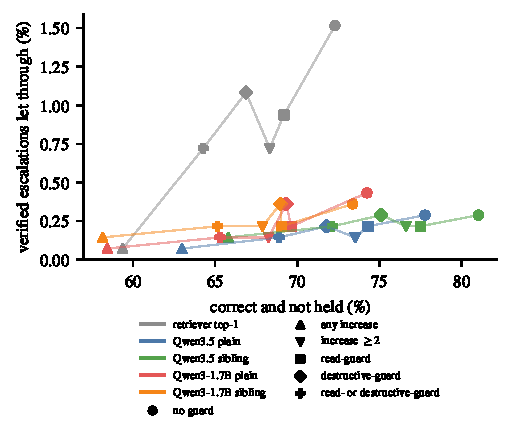
\includegraphics[width=\columnwidth]{../figs/tradeoff.pdf}
\caption{Verified escalation the guard would let through versus correct selections it would not hold,
under each guard policy (marker shape) and routing setup (colour), for retriever-only routing and LLM selection (\NumPoolTools{} tools).}
\label{fig:tradeoff}\end{figure}

\textbf{Answer to RQ3.} Side-effect metadata in the prompt changes little. Sibling expansion raises accuracy by 2.6 to 4.5 points for
the larger selectors. For Gemma3 and Phi-4 a plain shortlist of the same length does no better than
the top five, so length alone does not explain the gain; only for Qwen3.5 does it recover most of it. Neither changes escalation measurably. A guard is the only intervention that
removes most escalation, at the price of holding 15--20\,\% of calls for confirmation.

\subsection{Robustness: terse requests}
Our requests are explicit by construction, so we rewrote each one as a busy user would type it
(Qwen3.5, at most twelve words, no identifiers; mean \TerseWords{} words) and re-validated the
rewrites with Gemma3 among the siblings, keeping \TerseN. Terse requests are harder for every
stage: retriever-only top-1 accuracy at \NumPoolTools{} tools falls from \RetQwenPoolAcc\,\% to
\RetTQwenPoolAcc\,\%, and Qwen3.5's accuracy from \SelQPlainPoolAcc\,\% to \TerseQPlainAcc\,\%.
Terse escalation flags have not been human-labeled, so we report automatic rates only:
\GRTNoneSeer\,\% for the retriever's top hit and \TerseQPlainSeer\,\% after Qwen3.5 selection.
Sibling expansion still raises Qwen3.5's accuracy ($+2.3$ points) but now
\emph{lowers} Qwen3-1.7B's ($-3.1$ points). The any-increase guard holds
\GRTAnyHeld\,\% of retriever-only calls, close to its cost on explicit requests. Automatic rates rise
for terse requests (\GRTNoneSeer\,\% vs.\ \GRNonePoolExec\,\%), but automatic flags are mostly false, so whether
real escalation rises is open until the terse flags are labeled.
